%%%%%%%%%%%%%%%%%%%%%%%%%%%%%%%%%%%%%%%%%%%%%%%%%%%%%%%%%%%%%%%%
%                                                              %
% This is a LaTeX file.  It is a text file that is compiled    %
% by a program called LaTeX into a pretty PDF file.            %
% If you're viewing this file on Overleaf,                     %
% you'll see that PDF in the window to the right.              %
%                                                              %
% The LaTeX macro language is complicated, so we have inserted %
% lots of documenting comments into the file.  Comments start  %
% with `%' and continue to the end of the line.                %
%                                                              %
% Comments are provided to let you, the student, understand    %
% what that part of the code is doing or to provide you with   %
% instructions.                                                % 
%                                                              %
% Skip anything else you don't understand, or ask me.          %
%                                                              %
%%%%%%%%%%%%%%%%%%%%%%%%%%%%%%%%%%%%%%%%%%%%%%%%%%%%%%%%%%%%%%%%
%
\documentclass{article}
\usepackage[left=1in,right=1in,top=1in,bottom=1in]{geometry}
% 
%%%%%%%%%%%%%%%%%%%%%%%%%%%%%%%%%%%%%%%%%%%%%%%%%%%%%%%%%%%%%%%%
%                                                              %
% This is the preamble of the document. This is where we       %
% declare the packages we need for the pdf file to compile     %
% correctly. Packages contain the different commands we        %
% need to use that allow us to format the document nicely.     %
%                                                              %
% You shouldn't need to edit any of these packages.            %
%                                                              %
%%%%%%%%%%%%%%%%%%%%%%%%%%%%%%%%%%%%%%%%%%%%%%%%%%%%%%%%%%%%%%%%
% 
\usepackage{amsmath, amsthm, amsfonts} % These packages contain most of the commands needed to format the maths symbols.
\usepackage{enumerate} % Package that contains options for the \begin{enumerate} environment.
\usepackage{hyperref} % Package that allows hyperlinks.
\usepackage[nomessages]{fp} % This package allows LaTeX to do arithemtic based on defined parameters.
\usepackage{tikz} %  % tikz is the package ued to draw diagrams in LaTeX.
\newcommand{\NODE}[2]{\node[draw,circle,fill=white] (#1) at (#2) {};} % These three commands are for use with problem 4.
\newcommand{\BOX}{\draw (-3/2,3/2) -- (5/2,3/2) -- (5/2,-3/2) -- (-3/2,-3/2) -- (-3/2,3/2);}
\newcommand{\DRAWINGPROBLEM}{\foreach \n in {1,3,5}{\FPeval{\N}{round(\n+1,0)}
\node[draw,circle,fill=white] ({\n}) at ({-2*cos(-((\n-1)/2)*pi/3 r)},{2*sin(-((\n-1)/2)*pi/3 r)}) {$\n$};
\node[draw,circle,fill=white] ({\N}) at ({-2*cos((\N/2)*pi/3 r)},{2*sin((\N/2)*pi/3 r)}) {$\N$};}}
\newtheorem*{theorem}{Theorem} % Defines an environment with the heading "Theorem". The * supresses the numbering.
\newtheorem*{claim}{Claim} % Defines an environment with the heading "Claim". The * supresses the numbering.
\theoremstyle{definition}
\newtheorem*{definition}{Definition} % Defines an environment with the heading "Definition". The * supresses the numbering.
\newenvironment{solution}{\bigskip\hrule{\hfill}}{\bigskip\hrule{\hfill}} % Defines an environment that draws lines to make clear where your solution starts and ends.
% 
%%%%%%%%%%%%%%%%%%%%%%%%%%%%%%%%%%%%%%%%%%%%%%%%%%%%%%%%%%%%%%%%
%                                                              %
% In the author command below, type in your name. The article  %
% class will produce a title page using the command \maketitle %
% containing the title of the document, the author name and    %
% the date.                                                    %
%                                                              %
%%%%%%%%%%%%%%%%%%%%%%%%%%%%%%%%%%%%%%%%%%%%%%%%%%%%%%%%%%%%%%%%
%
\title{\textbf{MATH-UA 120 Discrete Mathematics: \\ Problem Set 9}}
\author{%
    Queen Elizabeth % Change to your name!
}
\date{Due Monday, December 9th, 2024} % The due date of the assignment. All assignemets are dues at 11:59pm on the date listed
%
%%%%%%%%%%%%%%%%%%%%%%%%%%%%%%%%%%%%%%%%%%%%%%%%%%%%%%%%%%%%%%%%
%                                                              %
% The body of the document is typed in between the lines       %
% \begin{document} and \end{document}.                         %
%                                                              %
%%%%%%%%%%%%%%%%%%%%%%%%%%%%%%%%%%%%%%%%%%%%%%%%%%%%%%%%%%%%%%%%
%
\begin{document}
\maketitle % This command generate the title page information that was filled in in the preamble

\vfill

% The following are the asignment instructions. You should leave these alone and, after reading them, proceed to the problems.
\section*{Assignment Instructions}

\begin{itemize}
    \item These are to be written up in \LaTeX{} and turned in on Gradescope.
    \item \href{https://bit.ly/3yZ1C7Q}{\textbf{Click here to duplicate this \texttt{.tex} file in Overleaf}}.
    \item Write your solutions inside the \texttt{solution} environment.
    \item You are always encouraged to talk problems through with your peers and your instructor, but your write up should be done independently.
    \item Problems are graded on correctness and fluency.
    \item Unless stated otherwise, all calculations require justification.
    \item Some tutorials on how to use \LaTeX{} can be found \href{https://www.overleaf.com/learn/latex/Tutorials}{\underline{here}}. If you have any questions about \LaTeX{} commands you can always ask your instructor for advice.
\end{itemize}

\vfill

\section*{Statement on generative AI}

In this and other mathematics courses, you are expected to construct clear and concise mathematical arguments based on statements proven in our text and class notes. Large language models such as ChatGPT are unable to produce this kind of solution. They also frequently generate circular logic and outright false results.
 
You may use AI to summarise content, generate study plans, create problems, or do other study-related activities. You may not ask a chatbot to solve your quiz or homework problems, or do any assessment-related activities.
 
You may use AI tools to edit your grammar and punctuation, but remember that mathematical English is not the same as academic English in other disciplines. 

\vfill

\newpage

%%%%%%%%%%%%%%%%%%%%%%%%%%%%%%%%%%%%%%%%%%%%%%%%%%%%%%%%%%%%%%%%
%%%%%                       Problem 1                      %%%%%
%%%%%%%%%%%%%%%%%%%%%%%%%%%%%%%%%%%%%%%%%%%%%%%%%%%%%%%%%%%%%%%%

\section*{Problem 1}
Let $G$ and $H$ be graphs. We say that $G$ is \emph{isomorphic} to $H$ if there is a bijection from $f:V\left(G\right)\longrightarrow V\left(H\right)$ such that for all $a,b\in V\left(G\right)$ we have $a\sim b$, in $G$, if and only if $f\left(a\right)\sim f\left(b\right)$, in $H$. The function $f$ is called an \emph{isomorphism} from $G$ to $H$.
    \begin{enumerate}[a)] % The enumerate environment produces a numbered list of items. The [a)] ensures that the items are labelled with letters instead.
	\item Prove that isomorphic graphs have the same number of vertices. 
	\item Prove that if $f:G\longrightarrow H$ is an isomorphism and $v\in V\left(G\right)$, then the degree of $v$ in $G$ is equal to the degree of $f\left(v\right)$ in $H$.
	\item Prove that isomorphic graphs have the same number of edges.
    \end{enumerate}

\begin{solution}

% Type your solution to Problem 1 here.

\end{solution}

%%%%%%%%%%%%%%%%%%%%%%%%%%%%%%%%%%%%%%%%%%%%%%%%%%%%%%%%%%%%%%%%

\newpage

%%%%%%%%%%%%%%%%%%%%%%%%%%%%%%%%%%%%%%%%%%%%%%%%%%%%%%%%%%%%%%%%
%%%%%                       Problem 2                      %%%%%
%%%%%%%%%%%%%%%%%%%%%%%%%%%%%%%%%%%%%%%%%%%%%%%%%%%%%%%%%%%%%%%%

\section*{Problem 2}
Suppose $G$ is a subgraph of $H$.  Prove or disprove:
    \begin{enumerate}[a)] % The enumerate environment produces a numbered list of items. The [a)] ensures that the items are labelled with letters instead.
	\item $\alpha(G) \leq \alpha(H)$
	\item $\omega(G) \leq \omega(H)$
    \end{enumerate}
\begin{solution}

% Type your solution to Problem 2 here.

\end{solution}

%%%%%%%%%%%%%%%%%%%%%%%%%%%%%%%%%%%%%%%%%%%%%%%%%%%%%%%%%%%%%%%%

\newpage

%%%%%%%%%%%%%%%%%%%%%%%%%%%%%%%%%%%%%%%%%%%%%%%%%%%%%%%%%%%%%%%%
%%%%%                       Problem 3                      %%%%%
%%%%%%%%%%%%%%%%%%%%%%%%%%%%%%%%%%%%%%%%%%%%%%%%%%%%%%%%%%%%%%%%

\section*{Problem 3}
Let $G=(V, E)$ be a graph with $V=\{v_1, v_2, \dots, v_n\}$. Its \textbf{degree sequence} is the list of degrees of its vertices, arranged in non-increasing order. That is, the degree sequence of $G$ is $(d(v_1), d(v_2), \dots, d(v_n))$ with the vertices arranged such that $d(v_1)\geq  d(v_2) \geq \dots \geq d(v_n)$. Below are different lists of possible degree sequences. Determine whether each case can be a graph with $n$ vertices. If not, explain why not. If so, describe a graph with these degrees: is the graph a complete graph, a cycle, a path, contains specific subgraphs, connected, etc?
	\begin{enumerate}[a)] % The enumerate environment produces a numbered list of items. The [a)] ensures that the items are labelled with letters instead.
		\item $n=7$ and $(6, 5, 4, 3, 2, 1, 0)$
		\item $n=6$ and $(2, 2, 2, 2, 2, 2)$
		\item $n=6$ and $(3, 2, 2, 2, 2, 2)$
		\item $n=6$ and $(1, 1, 1, 1, 1, 1)$
		\item $n=6$ and $(5, 3, 3, 3, 3, 3)$
    \end{enumerate}
\begin{solution}

% Type your solution to Problem 3 here.

\end{solution}

%%%%%%%%%%%%%%%%%%%%%%%%%%%%%%%%%%%%%%%%%%%%%%%%%%%%%%%%%%%%%%%%

\newpage

%%%%%%%%%%%%%%%%%%%%%%%%%%%%%%%%%%%%%%%%%%%%%%%%%%%%%%%%%%%%%%%%
%%%%%                       Problem 4                      %%%%%
%%%%%%%%%%%%%%%%%%%%%%%%%%%%%%%%%%%%%%%%%%%%%%%%%%%%%%%%%%%%%%%%

\section*{Problem 4}
Let $G=\left(V,E\right)$ be a graph with $V=\{1,2,3,4,5,6\}$. In the figures below we show the graphs (up to isomorphism) of $G-1$, $G-2$ and so on, but we do not have the names on the vertices. The goal of this problem is to reconstruct the graph $G$.

\begin{center} % tikz is the package ued to draw diagrams in LaTeX.
    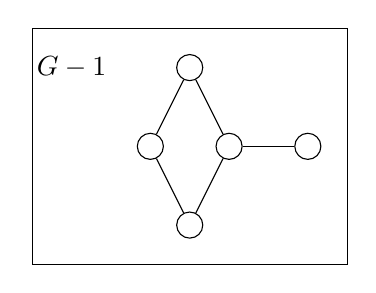
\begin{tikzpicture}	
    	\node at (-1, 1) {$G-1$}; \BOX \NODE{A}{0,0} \NODE{B}{1/2,1} \NODE{C}{1/2,-1} \NODE{D}{1,0} \NODE{E}{2,0}
       	\draw (A) -- (B) -- (D) -- (C) -- (A); \draw (D) -- (E);
	\end{tikzpicture}	\hspace*{1cm}
    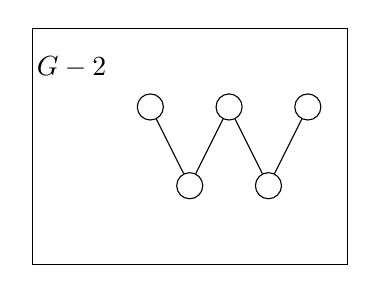
\begin{tikzpicture}	
    	\node at (-1, 1) {$G-2$}; \BOX \NODE{A}{0,1/2} \NODE{B}{1/2,-1/2} \NODE{C}{1,1/2} \NODE{D}{3/2,-1/2} \NODE{E}{2,1/2}
        \draw (A) -- (B) -- (C) -- (D) -- (E);
	\end{tikzpicture}	\hspace*{1cm}
    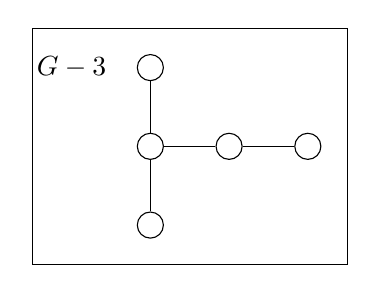
\begin{tikzpicture}	
    	\node at (-1, 1) {$G-3$}; \BOX \NODE{A}{0,1} \NODE{B}{0,0} \NODE{C}{0,-1} \NODE{D}{1,0} \NODE{E}{2,0}
        \draw (A) -- (B) -- (C); \draw (B) -- (D) -- (E);
	\end{tikzpicture}\\[15pt]
    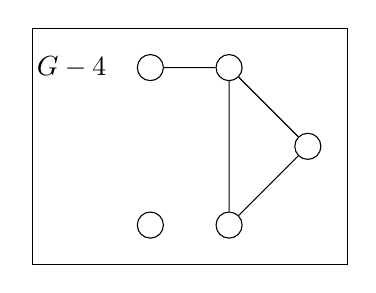
\begin{tikzpicture}
    	\node at (-1, 1) {$G-4$}; \BOX \NODE{A}{0,1} \NODE{B}{0,-1} \NODE{C}{1,1} \NODE{D}{1,-1} \NODE{E}{2,0}
        \draw (A) -- (C) -- (E) -- (D) -- (C);
	\end{tikzpicture}	\hspace*{1cm}
    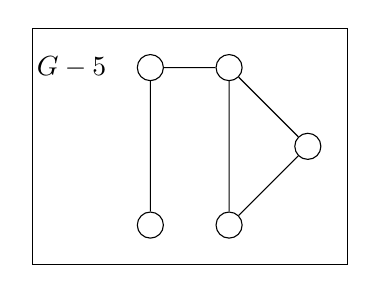
\begin{tikzpicture}
    	\node at (-1, 1) {$G-5$}; \BOX \NODE{A}{0,1} \NODE{B}{0,-1} \NODE{C}{1,1} \NODE{D}{1,-1} \NODE{E}{2,0}
        \draw (B) -- (A) -- (C) -- (E) -- (D) -- (C);
	\end{tikzpicture}	\hspace*{1cm}
    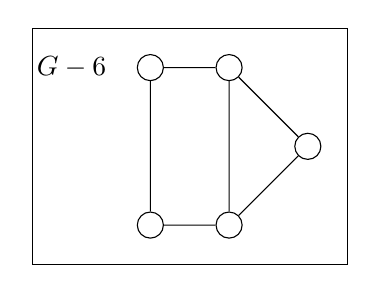
\begin{tikzpicture}	
    	\node at (-1, 1) {$G-6$}; \BOX \NODE{A}{0,1} \NODE{B}{0,-1} \NODE{C}{1,1} \NODE{D}{1,-1} \NODE{E}{2,0}
        \draw (D) -- (B) -- (A) -- (C) -- (E) -- (D) -- (C);
	\end{tikzpicture}
\end{center}

    \begin{enumerate}[a)] % The enumerate environment produces a numbered list of items. The [a)] ensures that the items are labelled with letters instead.
		\item Determine the number of edges in $G$.
		\item Using your answer in a) and the figures above, determine the degrees of each of the six vertices of $G$.
		\item Determine $G$ and sketch it. 
		
		\emph{There are instructions in the .tex file to help you draw the graph in \LaTeX.}
    \end{enumerate}    
    
\begin{solution}

% Type your solution to Problem 4 here.

% For part c), use the following code to help you draw the graph. Simply uncomment this section of code to get started.
% To uncomment a snippet of code in Overleaf, select/highlight the code snippet and press CMD + / (for Mac users) or CTRL + / (for Windows users)

%\begin{center}
%	\begin{tikzpicture} % tikz is the package ued to draw diagrams in LaTeX.
%    	\DRAWINGPROBLEM % This code was written to set you up with the six vertices. 
%    	% To draw the graph of your solution to this problem, you need only need draw the edges.
%    	% To draw an edge from a node labelled (A) to a node labelled (B), the command is \draw (A) -- (B);
%    	% The nodes in this graph have been labelled (1), (2), (3), (4), (5) and (6).
%    	% For example, the command 
%		%	\draw (1) -- (2); 
%		% draws a line connecting vertex 1 to vertex 2.
%    	% Another example, the command 
%		%	\draw (1) -- (2) -- (5) -- (1); 
%		% will draw a triangle, with vertices (1), (2) and (5).
%		% Write the code for each edge inside the tikzpicture environment.
%		% A semicolon is needed at the end of each line, or else you will get a compilation error.
%    	% If you find this too complicated, you can upload a hand-drawn picture using the \includegraphics command.
%    		
%
%    \end{tikzpicture}
%\end{center}

\end{solution}

%%%%%%%%%%%%%%%%%%%%%%%%%%%%%%%%%%%%%%%%%%%%%%%%%%%%%%%%%%%%%%%%

\newpage

%%%%%%%%%%%%%%%%%%%%%%%%%%%%%%%%%%%%%%%%%%%%%%%%%%%%%%%%%%%%%%%%
%%%%%                       Problem 5                      %%%%%
%%%%%%%%%%%%%%%%%%%%%%%%%%%%%%%%%%%%%%%%%%%%%%%%%%%%%%%%%%%%%%%%

\section*{Problem 5}
\begin{enumerate}[a)] % The enumerate environment produces a numbered list of items. The [a)] ensures that the items are labelled with letters instead.
	\item Given a graph with $n$ vertices. First, what is the maximum number of edges can the graph have and be disconnected? Then, what is the minimum number of edges we need to add to the previous graph to be connected?
	\item A \emph{complete bipartite graph} $K_{m,n}$ is a graph whose vertices can be partitioned $V=X\cup Y$ such that $|X|=m$ and  $|Y|=n$ for positive integers $m,n$, and $\{x, y\}$ is an edge in $K_{m,n}$ if and only if $x\in X$ and $y\in Y$. What is the number of edges in $K_{m,n}$?
	\item Given a cycle graph $C_4$, how many possible subgraphs of $C_4$ can there be?
\end{enumerate}
\begin{solution}

% Type your solution to Problem 5 here.

\end{solution}

%%%%%%%%%%%%%%%%%%%%%%%%%%%%%%%%%%%%%%%%%%%%%%%%%%%%%%%%%%%%%%%%

\newpage

%%%%%%%%%%%%%%%%%%%%%%%%%%%%%%%%%%%%%%%%%%%%%%%%%%%%%%%%%%%%%%%%
%%%%%                       Problem 6                      %%%%%
%%%%%%%%%%%%%%%%%%%%%%%%%%%%%%%%%%%%%%%%%%%%%%%%%%%%%%%%%%%%%%%%

\section*{Problem 6}
Prove that given a graph with exactly two vertices of odd degree, there must be a path joining these two vertices.
\begin{solution}

% Type your solution to Problem 6 here.

\end{solution}

%%%%%%%%%%%%%%%%%%%%%%%%%%%%%%%%%%%%%%%%%%%%%%%%%%%%%%%%%%%%%%%%

\newpage

%%%%%%%%%%%%%%%%%%%%%%%%%%%%%%%%%%%%%%%%%%%%%%%%%%%%%%%%%%%%%%%%
%%%%%                       Problem 7                      %%%%%
%%%%%%%%%%%%%%%%%%%%%%%%%%%%%%%%%%%%%%%%%%%%%%%%%%%%%%%%%%%%%%%%

\section*{Problem 7}
Prove by induction on $n$: Given integer $n\geq 1$, if  $T$ is a tree with $n$ vertices, then $T$ has $n-1$ edges. 
\begin{solution}

% Type your solution to Problem 7 here.

\end{solution}

%%%%%%%%%%%%%%%%%%%%%%%%%%%%%%%%%%%%%%%%%%%%%%%%%%%%%%%%%%%%%%%%

\newpage

%%%%%%%%%%%%%%%%%%%%%%%%%%%%%%%%%%%%%%%%%%%%%%%%%%%%%%%%%%%%%%%%
%%%%%                       Problem 8                      %%%%%
%%%%%%%%%%%%%%%%%%%%%%%%%%%%%%%%%%%%%%%%%%%%%%%%%%%%%%%%%%%%%%%%

\section*{Problem 8}
\begin{enumerate}[a)] % The enumerate environment produces a numbered list of items. The [a)] ensures that the items are labelled with letters instead.
	\item Prove that if a tree has $n$ vertices where $n\geq 4$ and is not a path graph $P_n$, then it has at least three vertices of degree 1.
	\item A \textbf{complete bipartite graph} $K_{m,n}$ is a graph whose vertices can be partitioned $V=X\cup Y$ such that $|X|=m$ and  $|Y|=n$ for positive integers $m,n$, and $\{x, y\}$ is an edge in $K_{m,n}$ if and only if $x\in X$ and $y\in Y$. Prove that every cycle in $K_{m, n}$ has an even number of edges.
\end{enumerate}
\begin{solution}

% Type your solution to Problem 8 here.

\end{solution}

%%%%%%%%%%%%%%%%%%%%%%%%%%%%%%%%%%%%%%%%%%%%%%%%%%%%%%%%%%%%%%%%

\newpage

%%%%%%%%%%%%%%%%%%%%%%%%%%%%%%%%%%%%%%%%%%%%%%%%%%%%%%%%%%%%%%%%
%%%%%                       Problem 9                      %%%%%
%%%%%%%%%%%%%%%%%%%%%%%%%%%%%%%%%%%%%%%%%%%%%%%%%%%%%%%%%%%%%%%%

\section*{Problem 9}
Given a tree $G$ with two vertices of degree 2, four vertices of degree 3, three vertices of degree 4, and the remaining vertices of degree 1. How many vertices does $G$ have?    
\begin{solution}

% Type your solution to Problem 9 here.

\end{solution}

%%%%%%%%%%%%%%%%%%%%%%%%%%%%%%%%%%%%%%%%%%%%%%%%%%%%%%%%%%%%%%%%

\end{document}
%
% Anything typed after \end{document} will not be included in the pdf


